\documentclass[conference]{IEEEtran}
\IEEEoverridecommandlockouts
% The preceding line is only needed to identify funding in the first footnote. If that is unneeded, please comment it out.
%Template version as of 6/27/2024

\usepackage[spanish,mexico]{babel}
\usepackage{verbatim}
\usepackage{longtable,multirow,booktabs}
\usepackage{url}

%\usepackage{cite}
\usepackage{amsmath,amssymb,amsfonts}
\usepackage{algorithmic}
\usepackage{graphicx}
\usepackage{textcomp}
%\usepackage{biblatex}
\usepackage{xcolor}

\usepackage{csquotes}
\usepackage{float}
\usepackage{multicol}

\usepackage[backend=biber,style=ieee]{biblatex}
\addbibresource{biblio.bib}

\def\BibTeX{{\rm B\kern-.05em{\sc i\kern-.025em b}\kern-.08em
    T\kern-.1667em\lower.7ex\hbox{E}\kern-.125emX}}

    


\begin{document}

\title{Análisis macro económico: \\ 
{\LARGE 2000 - 2023}
%\thanks{Identify applicable funding agency here. If none, delete this.}
}

\author{\IEEEauthorblockN{Ilian Montserrat Garza Aguirre \quad Rey Alexis Salas-Vega}
\IEEEauthorblockA{\textit{Visualización de Datos} \\
\textit{Dra. Valeria Soto Mendoza}\\
\textit{Maestría en Ciencia de Datos y Optimización}\\
\textit{CIMA, UA de C}\\
Saltillo, Coah., México \\
garzailian@uadec.edu.mx \quad rey.vega@uadec.edu.mx}}
% \and
% \IEEEauthorblockN{2\textsuperscript{nd} Given Name Surname}
% \IEEEauthorblockA{\textit{dept. name of organization (of Aff.)} \\
% \textit{name of organization (of Aff.)}\\
% City, Country \\
% email address or ORCID}}
% \and
% \IEEEauthorblockN{3\textsuperscript{rd} Given Name Surname}
% \IEEEauthorblockA{\textit{dept. name of organization (of Aff.)} \\
% \textit{name of organization (of Aff.)}\\
% City, Country \\
% email address or ORCID}
% \and
% \IEEEauthorblockN{4\textsuperscript{th} Given Name Surname}
% \IEEEauthorblockA{\textit{dept. name of organization (of Aff.)} \\
% \textit{name of organization (of Aff.)}\\
% City, Country \\
% email address or ORCID}
% \and
% \IEEEauthorblockN{5\textsuperscript{th} Given Name Surname}
% \IEEEauthorblockA{\textit{dept. name of organization (of Aff.)} \\
% \textit{name of organization (of Aff.)}\\
% City, Country \\
% email address or ORCID}
% \and
% \IEEEauthorblockN{6\textsuperscript{th} Given Name Surname}
% \IEEEauthorblockA{\textit{dept. name of organization (of Aff.)} \\
% \textit{name of organization (of Aff.)}\\
% City, Country \\
% email address or ORCID}
% }
%%%%%%%%%%%%%%%%%%%%%%%%%%%%%%%%%%%%%%%%%%%%%%%%%%%%%%%%%%%%%%%%%%%%%%%%%%%%%%%%%%%%%%%%%%%%%%%%%%%%%%%%%%%%%%%%%%%%%%%%%%%
\maketitle

%%%%%%%%%%%%%%%%%%%%%%%%%%%%%%%%%%%%%%%%%%%%%%%%%%%%%%%%%%%%%%%%%%%%%%%%%%%%%%%%%%%%%%%%%%%%%%%%%%%%%%%%%%%%%%%%%%%%%%%%%%%
\begin{abstract}

\end{abstract}

\begin{IEEEkeywords}
COVID-19, 
\end{IEEEkeywords}

%%%%%%%%%%%%%%%%%%%%%%%%%%%%%%%%%%%%%%%%%%%%%%%%%%%%%%%%%%%%%%%%%%%%%%%%%%%%%%%%%%%%%%%%%%%%%%%%%%%%%%%%%%%%%%%%%%%%%%%%%%%
\section{Introducción}

Tras el surgimiento del virus del COVID-19 y su rápida propagación, se tomaron estrictas medidas de contención por parte de las naciones, transformando las relaciones comerciales, sociales, políticas y espaciales, provocando distanciamiento social, paro productivo e interrupción de las cadenas de suministro \cite{espitia2022}, además del surgimiento de nuevas necesidades, generadas a partir del sometimiento de los seres humanos a nuevas realidades \cite{djokic2022}. 

%%%%%%%%%%%%%%%%%%%%%%%%%%%%%%%%%%%%%%%%%%%%%%%%%%%%%%%%%%%%%%
\section{Caso de estudio}

A manera de analizar los efectos económicos causados por la pandemia de COVID-19 en distintas naciones del mundo, se plantea un caso de estudio, a partir del cual se busca estudiar el comportamiento de un conjunto de datos correspondiente a 6 variables macro económicas. 

Presentando el escenario en el cual un conjunto de 109 países acuden al Banco Mundial en busca de ayuda para dimensionar el impacto de los estragos económicos a causa de la pandemia por COVID-19, y así posterior al análisis estadístico descriptivo proporcionado por la institución, las naciones sean capaces de diseñar políticas públicas las cuales permitan brindar un aumento de bienestar social a su población.

%%%%%%%%%%%%%%%%%%%%%%%%%%%%%%%%%%%%%%%%%%%%%%%%%%%%%%%%%%%%%
\section{Base de datos}

La muestra empleada para el desarrollo de la presente investigación se compone de dos segmentos de datos, en una primera instancia se presentan los datos obtenidos de manera tradicional referente a 109 naciones del año 2000 al 2023, correspondientes a nuestra variable dependiente (variable objetivo) y variables independientes (sus determinantes), los cuales fueron obtenidos a través del portal de datos abiertos del Banco Mundial \cite{worldbank}.

Como parte de nuestro análisis de recuperación económica post-COVID, nuestra base incluye la categorización de los países que la conforman mediante el grupo de ingreso al cual pertenecen, tal como se muestra en la figura \ref{fig:mapa}. 

\begin{figure}[H]
    \centering
    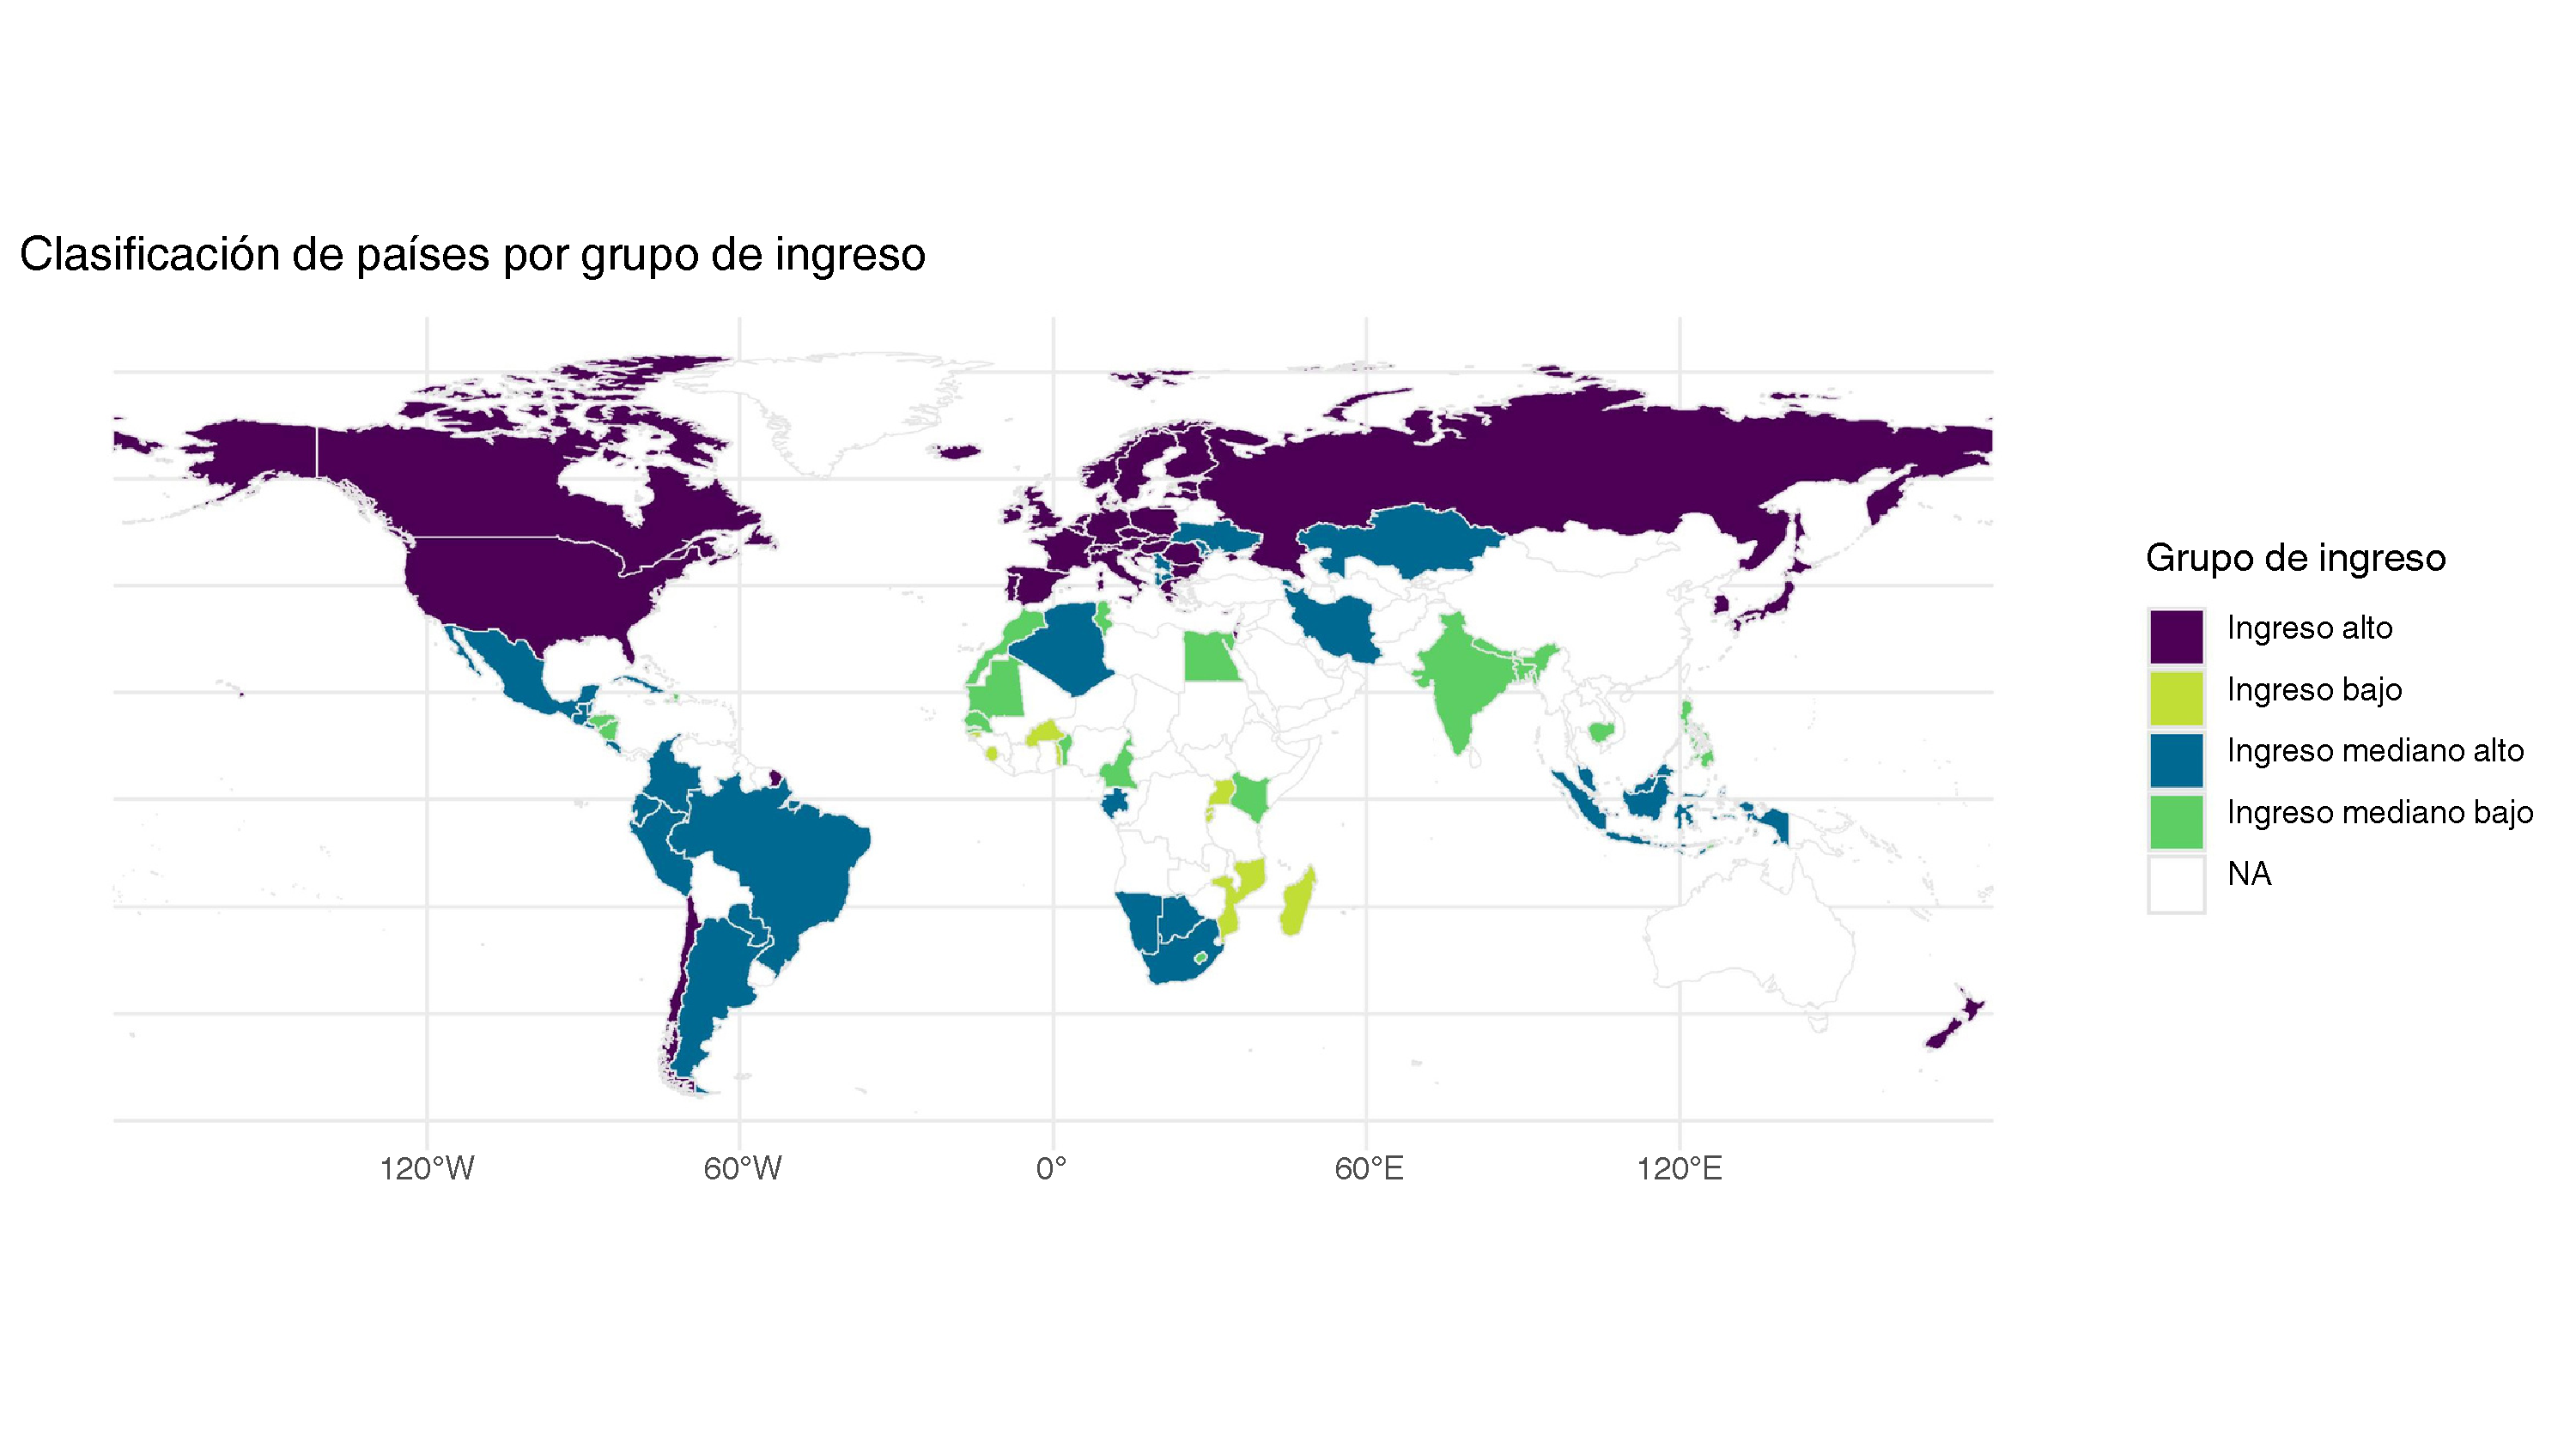
\includegraphics[width=1.1\linewidth]{Paisesingreso.pdf}
    \caption{Clasificación de los países que integran la base categorizados por grupo de ingreso}
    \label{fig:mapa}
\end{figure}

La categorización de cada país es efectuada por el Banco Mundial y la manera en la que se realiza la asignación de cada país es a través de intervalos en base al ingreso nacional bruto per cápita de cada país de cada año, al que se le realiza un ajuste inflacionario utilizando el deflactor de  derechos especiales de giro, para mantener fijos los umbrales de la clasificación por ingreso en términos reales.

Siendo los países de ingresos medianos bajos son aquellos con un INB per cápita entre 1,146 y 4,515, los de ingresos medianos altos son aquellos con un INB per cápita entre 4,516 y 14.005 dólares y los países de altos ingresos son aquellos con un INB per cápita de más de 14,005 dólares en 2023.

La clasificación de ingresos del Banco Mundial tiene como objetivo reflejar el nivel de desarrollo de un país, basándose en el INB per cápita calculado según el método Atlas como un indicador ampliamente disponible de la capacidad económica \cite{Worldbankblog}.

La selección de las variables, se realizo en base a la teoría keynesiana del consumo \cite{keynes1937}, la cual se desglosa de manera más precisa en el capítulo anterior, en donde se presenta la composición del producto de cualquier economía, a través de diversos componentes macro económicos, tomando la relación de dichos componentes de manera unilateral, el consumo se ve representado como ...
\begin{equation}
    C = PIB + I + G + (X - M)
\end{equation}

En donde el PIB (Producto Interno Bruto) representa al ingreso nacional, C es al consumo, I a la inversión, G al gasto público o de gobierno, X  las exportaciones y M  las importaciones.

Una vez recopilados los datos, se dio inicio su preprocesamiento, en donde las variables correspondientes al PIB, inversión y gasto público, se procedieron a dividir entre la población total y aquellas variables que conforman la balanza comercial, o sea, las exportaciones y las importaciones, se dividieron entre el PIB, esto como parte del proceso de preparación de datos, con la intención de reducir el sesgo demográfico presente entre las naciones, para posteriormente estructurarse en forma de panel, por fines de practicidad en el manejo, aplicación y análisis del modelo.

De igual manera, como parte del proceso de preparación de datos, se procedió a aplicar la técnica de estandarización de datos Min-max y que de esta manera no se presente una brecha tan amplia entre las escalas presentes en los datos de cada variable.

El escalado mín-máx es una técnica empleada para re escalar características de modo que se encuentren dentro de un rango específico, generalmente [0, 1], en la cual se aplica la siguiente.

\begin{equation}
    X_{\text{scaled}} = \frac{X - X_{\text{min}}}{X_{\text{max}} - X_{\text{min}}}
\end{equation}
%%%%%%%%%%%%%%%%%%%%%%%%%%%%%%%%%%%%%%%%%%%%%%%%%%%%%%%%%%%%%%%%%%%%%%%%%%%%%%%%%%%%%%%%%%%%%%%%%%%%%%%%%%%%%%%%%%%%%%%%%%%%%%%%%%%%%%%%%%%%%%%%%%%%%%%%%%%%%%%%%%%%%
\section{Resultados}

Un primer acercamiento al análisis descriptivo exploratorio de nuestro conjunto de datos, es por medio de la presentación de las estadísticas descriptivas correspondientes, las cuales se muestran en la tabla.

% Please add the following required packages to your document preamble:
% \usepackage{multirow}
% \begin{table}[ht]
% \tiny
% \begin{tabular}{|c|l|c|c|c|c|c|}
% \hline
% \multicolumn{1}{|l|}{Variable} &
%   Metrica &
%   \multicolumn{1}{l|}{General} &
%   \multicolumn{1}{l|}{Alto} &
%   \multicolumn{1}{l|}{Medio alto} &
%   \multicolumn{1}{l|}{Medio bajo} &
%   \multicolumn{1}{l|}{Bajo} \\ \hline
% \multirow{7}{*}{G}   & Media          & 0.1428942  & 0.32742663  & 4.83E-02  & 1.30E-02 & 4.14E-03  \\ \cline{2-7} 
%                      & Desv. estándar & 0.198231   & 0.21302744  & 2.78E-02  & 1.06E-02 & 1.96E-03  \\ \cline{2-7} 
%                      & C. variación   & 1.387258   & 0.65061124  & 2.78E-02  & 1.06E-02 & 4.75E-01  \\ \cline{2-7} 
%                      & Error estándar & 0.00387572 & 2.50E-02    & 4.27E-02  & 6.14E-02 & 5.84E-02  \\ \cline{2-7} 
%                      & Varianza       & 0.03929554 & 0.04538069  & 7.71E-04  & 1.13E-04 & 3.86E-06  \\ \cline{2-7} 
%                      & Skewness       & 1.791408   & 7.93E-01    & 1.15E+00  & 1.50E+00 & 9.92E-01  \\ \cline{2-7} 
%                      & Kurtosis       & 2.626699   & -0.03739892 & 2.02E+00  & 1.02E+00 & 2.23E+00  \\ \hline
% \multirow{7}{*}{C}   & Media          & 0.2035985  & 0.41450388  & 1.01E-01  & 5.23E-02 & 3.68E-02  \\ \cline{2-7} 
%                      & Desv. estándar & 0.2191341  & 0.22413832  & 3.24E-02  & 1.15E-02 & 2.63E-03  \\ \cline{2-7} 
%                      & C. variación   & 1.076305   & 0.54073879  & 3.21E-01  & 2.20E-01 & 7.14E-02  \\ \cline{2-7} 
%                      & Error estándar & 0.00428441 & 0.02077554  & 2.82E-02  & 3.78E-02 & 6.75E-03  \\ \cline{2-7} 
%                      & Varianza       & 0.04801974 & 0.05023799  & 1.05E-03  & 1.33E-04 & 6.91E-06  \\ \cline{2-7} 
%                      & Skewness       & 1.617019   & 0.65960307  & 7.57E-01  & 9.26E-01 & 1.15E-01  \\ \cline{2-7} 
%                      & Kurtosis       & 1.88622    & -0.25166801 & 1.14E+00  & 3.61E-01 & -2.33E-01 \\ \hline
% \multirow{7}{*}{I}   & Media          & 0.162402   & 0.25764895  & 1.15E-01  & 9.50E-02 & 8.83E-02  \\ \cline{2-7} 
%                      & Desv. estándar & 0.105916   & 0.11794690  & 1.77E-02  & 6.23E-03 & 1.57E-03  \\ \cline{2-7} 
%                      & C. variación   & 0.6521841  & 0.45778141  & 1.54E-01  & 6.55E-02 & 1.78E-02  \\ \cline{2-7} 
%                      & Error estándar & 0.00207082 & 0.04508185  & -2.70E-02 & 5.75E-02 & 8.06E-02  \\ \cline{2-7} 
%                      & Varianza       & 0.0112182  & 0.01391147  & 3.12E-04  & 3.88E-05 & 2.47E-06  \\ \cline{2-7} 
%                      & Skewness       & 2.195242   & 1.43130439  & -7.24E-01 & 1.41E+00 & 1.37E+00  \\ \cline{2-7} 
%                      & Kurtosis       & 5.906043   & 2.92119182  & 5.75E+00  & 2.82E+00 & 4.42E+00  \\ \hline
% \multirow{7}{*}{M}   & Media          & 0.3240234  & 0.36452218  & 3.02E-01  & 3.11E-01 & 2.64E-01  \\ \cline{2-7} 
%                      & Desv. estándar & 0.1203152  & 0.14496975  & 9.19E-02  & 1.01E-01 & 6.71E-02  \\ \cline{2-7} 
%                      & C. variación   & 0.3713162  & 0.39769802  & 3.04E-01  & 3.26E-01 & 2.55E-01  \\ \cline{2-7} 
%                      & Error estándar & 0.00235235 & 0.04998721  & 1.46E-02  & 4.65E-02 & 1.05E-01  \\ \cline{2-7} 
%                      & Varianza       & 0.01447574 & 0.02101623  & 8.45E-03  & 1.03E-02 & 4.51E-03  \\ \cline{2-7} 
%                      & Skewness       & 1.681117   & 1.5870447   & 3.92E-01  & 1.14E+00 & 1.78E+00  \\ \cline{2-7} 
%                      & Kurtosis       & 4.51881    & 3.02756078  & -4.86E-01 & 1.56E+00 & 6.34E+00  \\ \hline
% \multirow{7}{*}{X}   & Media          & 0.1804222  & 0.2518417   & 1.60E-01  & 1.28E-01 & 9.12E-02  \\ \cline{2-7} 
%                      & Desv. estándar & 0.1301678  & 0.15817314  & 8.35E-02  & 8.37E-02 & 4.30E-02  \\ \cline{2-7} 
%                      & C. variación   & 0.721462   & 0.62806572  & 5.23E-01  & 6.53E-01 & 4.72E-01  \\ \cline{2-7} 
%                      & Error estándar & 0.00254498 & 0.06078777  & 4.66E-02  & 4.37E-02 & 1.65E-02  \\ \cline{2-7} 
%                      & Varianza       & 0.01694365 & 0.02501874  & 6.97E-03  & 7.00E-03 & 1.85E-03  \\ \cline{2-7} 
%                      & Skewness       & 2.246592   & 1.92995194  & 1.25E+00  & 1.07E+00 & 2.80E-01  \\ \cline{2-7} 
%                      & Kurtosis       & 7.900132   & 4.75760923  & 1.65E+00  & 1.24E+00 & -3.60E-01 \\ \hline
% \multirow{7}{*}{PIB} & Media          & 0.1292762  & 0.29209467  & 2.97E-03  & 4.88E-02 & 1.30E-02  \\ \cline{2-7} 
%                      & Desv. estándar & 0.1762393  & 0.19089998  & 2.33E-02  & 7.75E-03 & 1.75E-03  \\ \cline{2-7} 
%                      & C. variación   & 1.363277   & 0.65355517  & 4.77E-01  & 5.98E-01 & 5.88E-01  \\ \cline{2-7} 
%                      & Error estándar & 0.00344575 & 0.03912028  & 3.56E-02  & 4.25E-02 & 2.74E-02  \\ \cline{2-7} 
%                      & Varianza       & 0.03106029 & 0.0364428   & 5.41E-04  & 6.01E-05 & 3.05E-06  \\ \cline{2-7} 
%                      & Skewness       & 2.024297   & 1.24203044  & 9.54E-01  & 1.04E+00 & 4.64E-01  \\ \cline{2-7} 
%                      & Kurtosis       & 4.47265    & 1.78959581  & 7.08E-01  & 2.07E-01 & -1.20E-01 \\ \hline
% \end{tabular}
% \end{table}

\begin{table}[H]
    \tiny
    \centering
    \begin{tabular}{|c|l|c|c|c|c|c|}
\hline
\multicolumn{1}{|l|}{Variable} &
  Metrica &
  \multicolumn{1}{l|}{General} &
  \multicolumn{1}{l|}{Alto} &
  \multicolumn{1}{l|}{Medio alto} &
  \multicolumn{1}{l|}{Medio bajo} &
  \multicolumn{1}{l|}{Bajo} \\ \hline
\multirow{7}{*}{G}   & Media          & 1.43E-01  & 3.27E-01  & 4.83E-02  & 1.30E-02 & 4.14E-03  \\ \cline{2-7} 
                     & Desv. estándar & 1.98E-01  & 2.13E-01  & 2.78E-02  & 1.06E-02 & 1.96E-03  \\ \cline{2-7} 
                     & C. variación   & 1.39E+00  & 6.51E-01  & 2.78E-02  & 1.06E-02 & 4.75E-01  \\ \cline{2-7} 
                     & Error estándar & 3.88E-03  & 2.50E-02  & 4.27E-02  & 6.14E-02 & 5.84E-02  \\ \cline{2-7} 
                     & Varianza       & 3.93E-02  & 4.54E-02  & 7.71E-04  & 1.13E-04 & 3.86E-06  \\ \cline{2-7} 
                     & Skewness       & 1.79E+00  & 7.93E-01  & 1.15E+00  & 1.50E+00 & 9.92E-01  \\ \cline{2-7} 
                     & Kurtosis       & 2.63E+00  & -3.74E-02 & 2.02E+00  & 1.02E+00 & 2.23E+00  \\ \hline
\multirow{7}{*}{C}   & Media          & 2.04E-01  & 4.15E-01  & 1.01E-01  & 5.23E-02 & 3.68E-02  \\ \cline{2-7} 
                     & Desv. estándar & 2.19E-01  & 2.24E-01  & 3.24E-02  & 1.15E-02 & 2.63E-03  \\ \cline{2-7} 
                     & C. variación   & 1.08E+00  & 5.41E-01  & 3.21E-01  & 2.20E-01 & 7.14E-02  \\ \cline{2-7} 
                     & Error estándar & 4.28E-03  & 2.08E-02  & 2.82E-02  & 3.78E-02 & 6.75E-03  \\ \cline{2-7} 
                     & Varianza       & 4.80E-02  & 5.02E-02  & 1.05E-03  & 1.33E-04 & 6.91E-06  \\ \cline{2-7} 
                     & Skewness       & 1.62E+00  & 6.60E-01  & 7.57E-01  & 9.26E-01 & 1.15E-01  \\ \cline{2-7} 
                     & Kurtosis       & 1.89E+00  & -2.52E-01 & 1.14E+00  & 3.61E-01 & -2.33E-01 \\ \hline
\multirow{7}{*}{I}   & Media          & 1.62E-01  & 2.58E-01  & 1.15E-01  & 9.50E-02 & 8.83E-02  \\ \cline{2-7} 
                     & Desv. estándar & 1.06E-01  & 1.18E-01  & 1.77E-02  & 6.23E-03 & 1.57E-03  \\ \cline{2-7} 
                     & C. variación   & 6.52E-01  & 4.58E-01  & 1.54E-01  & 6.55E-02 & 1.78E-02  \\ \cline{2-7} 
                     & Error estándar & 2.07E-03  & 4.51E-02  & -2.70E-02 & 5.75E-02 & 8.06E-02  \\ \cline{2-7} 
                     & Varianza       & 1.12E-02  & 1.39E-02  & 3.12E-04  & 3.88E-05 & 2.47E-06  \\ \cline{2-7} 
                     & Skewness       & 2.20E+00  & 1.43E+00  & -7.24E-01 & 1.41E+00 & 1.37E+00  \\ \cline{2-7} 
                     & Kurtosis       & 5.91E+00  & 2.92E+00  & 5.75E+00  & 2.82E+00 & 4.42E+00  \\ \hline
\multirow{7}{*}{M}   & Media          & 3.24E-01  & 3.65E-01  & 3.02E-01  & 3.11E-01 & 2.64E-01  \\ \cline{2-7} 
                     & Desv. estándar & 1.20E-01  & 1.45E-01  & 9.19E-02  & 1.01E-01 & 6.71E-02  \\ \cline{2-7} 
                     & C. variación   & 3.71E-01  & 3.98E-01  & 3.04E-01  & 3.26E-01 & 2.55E-01  \\ \cline{2-7} 
                     & Error estándar & 2.35E-03  & 5.00E-02  & 1.46E-02  & 4.65E-02 & 1.05E-01  \\ \cline{2-7} 
                     & Varianza       & 1.45E-02  & 2.10E-02  & 8.45E-03  & 1.03E-02 & 4.51E-03  \\ \cline{2-7} 
                     & Skewness       & 1.68E+00  & 1.59E+00  & 3.92E-01  & 1.14E+00 & 1.78E+00  \\ \cline{2-7} 
                     & Kurtosis       & 4.52E+00  & 3.03E+00  & -4.86E-01 & 1.56E+00 & 6.34E+00  \\ \hline
\multirow{7}{*}{X}   & Media          & 1.80E-01  & 2.52E-01  & 1.60E-01  & 1.28E-01 & 9.12E-02  \\ \cline{2-7} 
                     & Desv. estándar & 1.30E-01  & 1.58E-01  & 8.35E-02  & 8.37E-02 & 4.30E-02  \\ \cline{2-7} 
                     & C. variación   & 7.21E-01  & 6.28E-01  & 5.23E-01  & 6.53E-01 & 4.72E-01  \\ \cline{2-7} 
                     & Error estándar & 2.54E-03  & 6.08E-02  & 4.66E-02  & 4.37E-02 & 1.65E-02  \\ \cline{2-7} 
                     & Varianza       & 1.69E-02  & 2.50E-02  & 6.97E-03  & 7.00E-03 & 1.85E-03  \\ \cline{2-7} 
                     & Skewness       & 2.25E+00  & 1.93E+00  & 1.25E+00  & 1.07E+00 & 2.80E-01  \\ \cline{2-7} 
                     & Kurtosis       & 7.90E+00  & 4.76E+00  & 1.65E+00  & 1.24E+00 & -3.60E-01 \\ \hline
\multirow{7}{*}{PIB} & Media          & 1.29E-01  & 2.92E-01  & 2.97E-03  & 4.88E-02 & 1.30E-02  \\ \cline{2-7} 
                     & Desv. estándar & 1.76E-01  & 1.91E-01  & 2.33E-02  & 7.75E-03 & 1.75E-03  \\ \cline{2-7} 
                     & C. variación   & 1.36E+00  & 6.54E-01  & 4.77E-01  & 5.98E-01 & 5.88E-01  \\ \cline{2-7} 
                     & Error estándar & 3.45E-03  & 3.91E-02  & 3.56E-02  & 4.25E-02 & 2.74E-02  \\ \cline{2-7} 
                     & Varianza       & 3.11E-02  & 3.64E-02  & 5.41E-04  & 6.01E-05 & 3.05E-06  \\ \cline{2-7} 
                     & Skewness       & 2.02E+00  & 1.24E+00  & 9.54E-01  & 1.04E+00 & 4.64E-01  \\ \cline{2-7} 
                     & Kurtosis       & 4.47E+00  & 1.79E+00  & 7.08E-01  & 2.07E-01 & -1.20E-01 \\ \hline
\end{tabular}

\end{table}

De igual manera, resulta relevante la representación visual del comportamiento de nuestras variables a través de series de tiempo como parte de este análisis.

\begin{figure}[H]
    \centering
    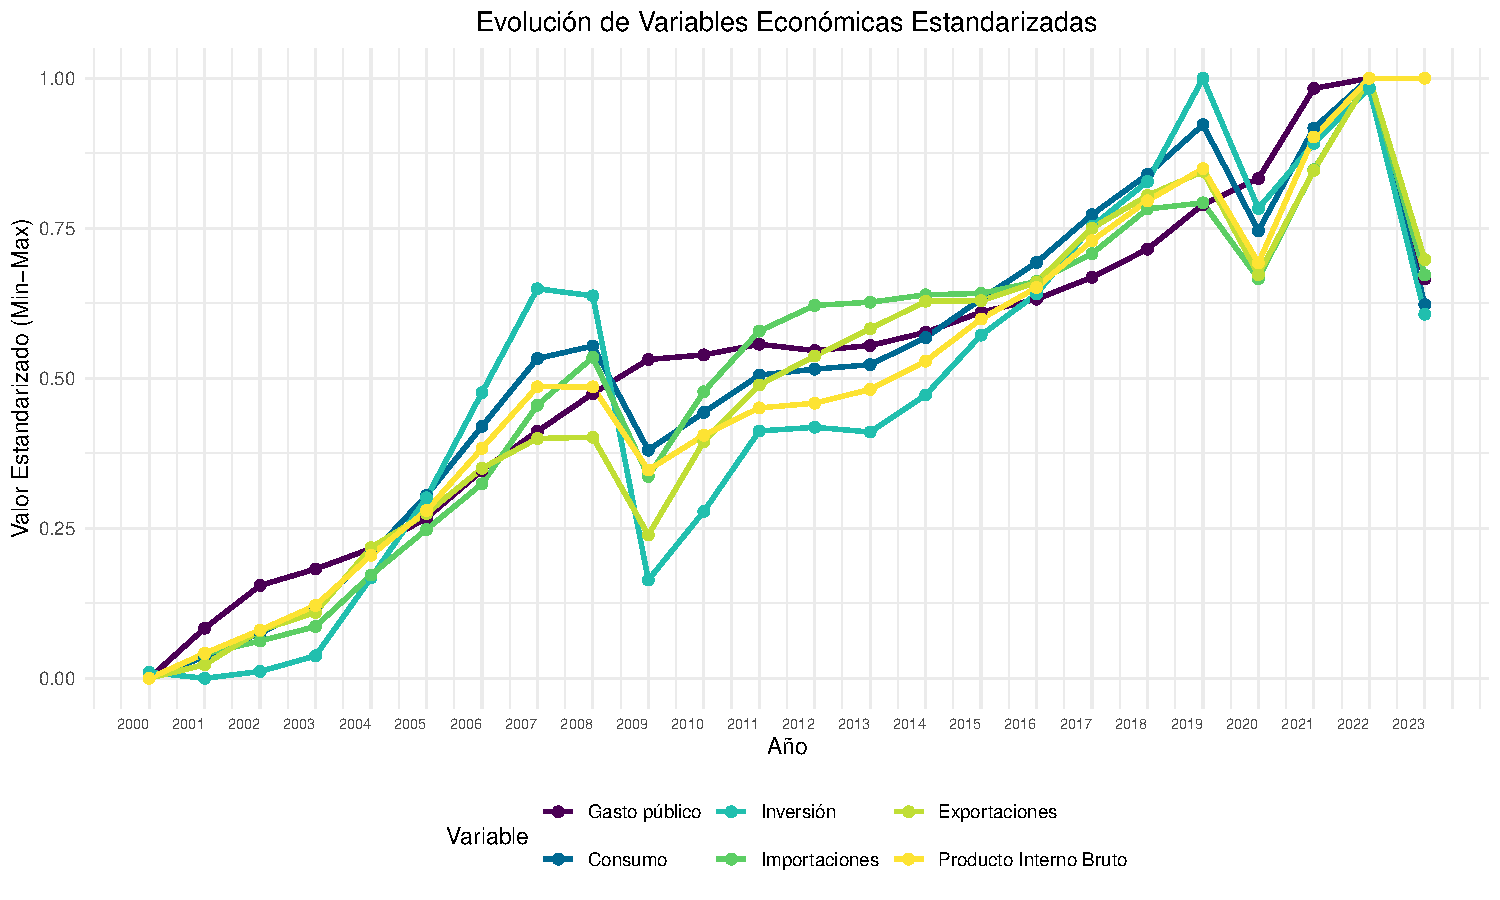
\includegraphics[width=1\linewidth]{figures/graficotot.pdf}
    \caption{Comportamiento de las variables a través del tiempo a nivel global}
    \label{fig:serietot}
\end{figure}

\begin{figure}[H]
    \centering
    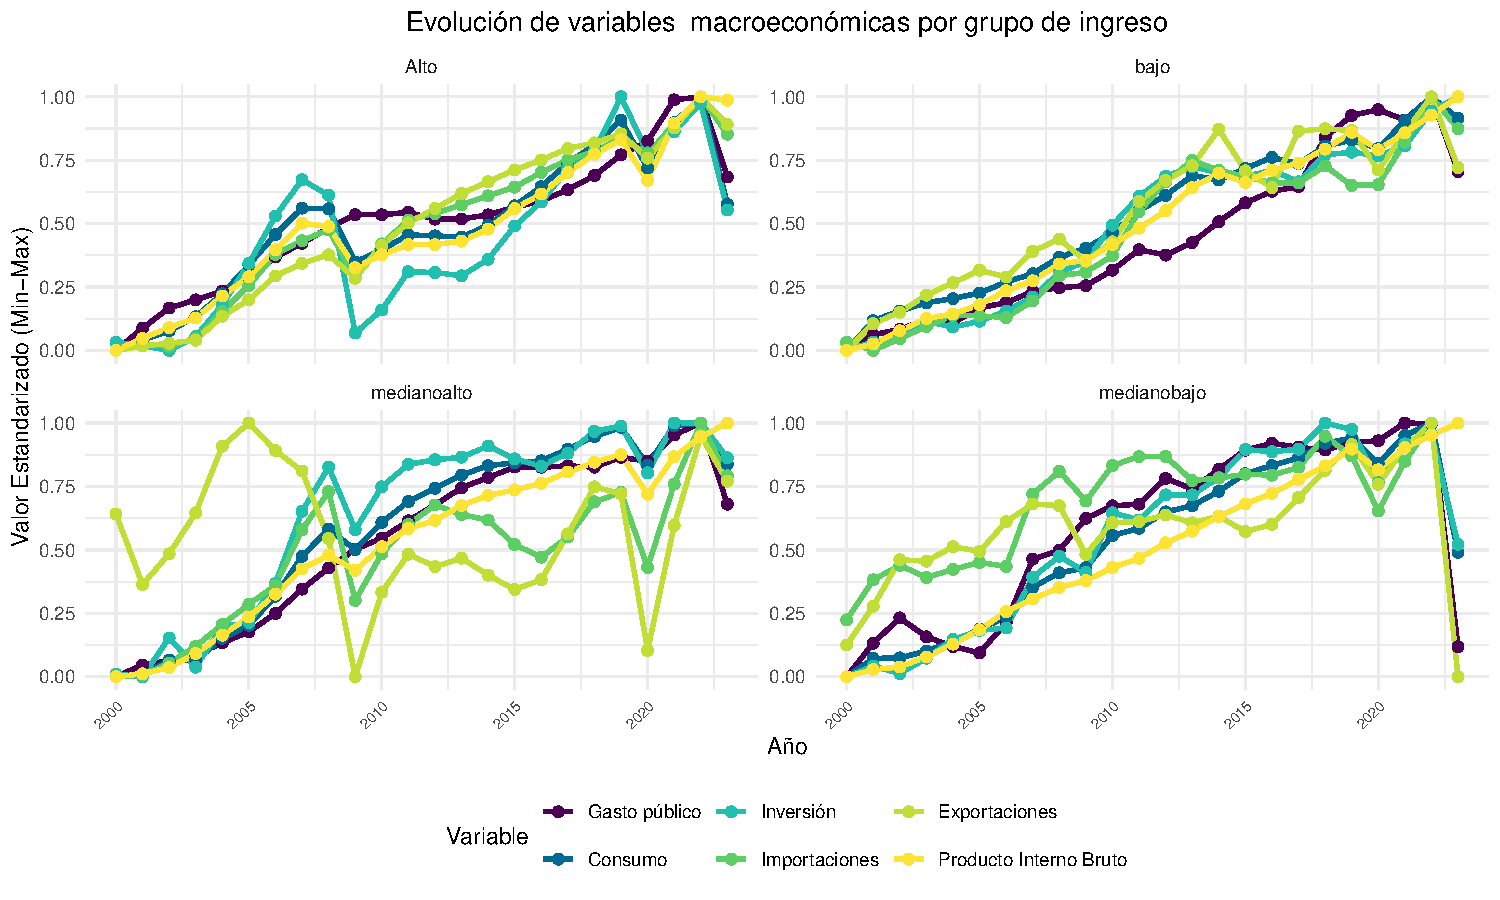
\includegraphics[width=1\linewidth]{figures/mi_grafico.pdf}
    \caption{Comportamiento de las variables a través del tiempo según su grupo de ingreso}
    \label{fig:serieing}
\end{figure}

En una primera instancia se muestra el comportamiento de las variables macroeconómicas de manera conjunta para los 109 países en la figura \ref{fig:serietot}, para posteriormente mostrarse el comportamiento de dichas variables categorizadas según el grupo de ingreso al que pertenece cada país \ref{fig:serieing}.

En caso de desear visualizar las modificaciones de las variables por país a través del tiempo, se incentiva a los lectores a visitar \url{https://github.com/rasv2000/Proyecto_DataViz}, en donde se muestra un dashboard que incluye mapas y series de tiempo interactivos para cada variable y cada país que conforman la muestra.

Una vez visualizado el comportamiento de nuestras variables, es posible intuir que nuestro conjunto de datos tiene un comportamiento no estacionario, o sea que son no paramétricos, sin embargo, es necesaria la aplicación pruebas de normalidad, así como la visualización de su distribución para la comprobación de dicha sospecha.

\begin{figure}[H]
    \centering
    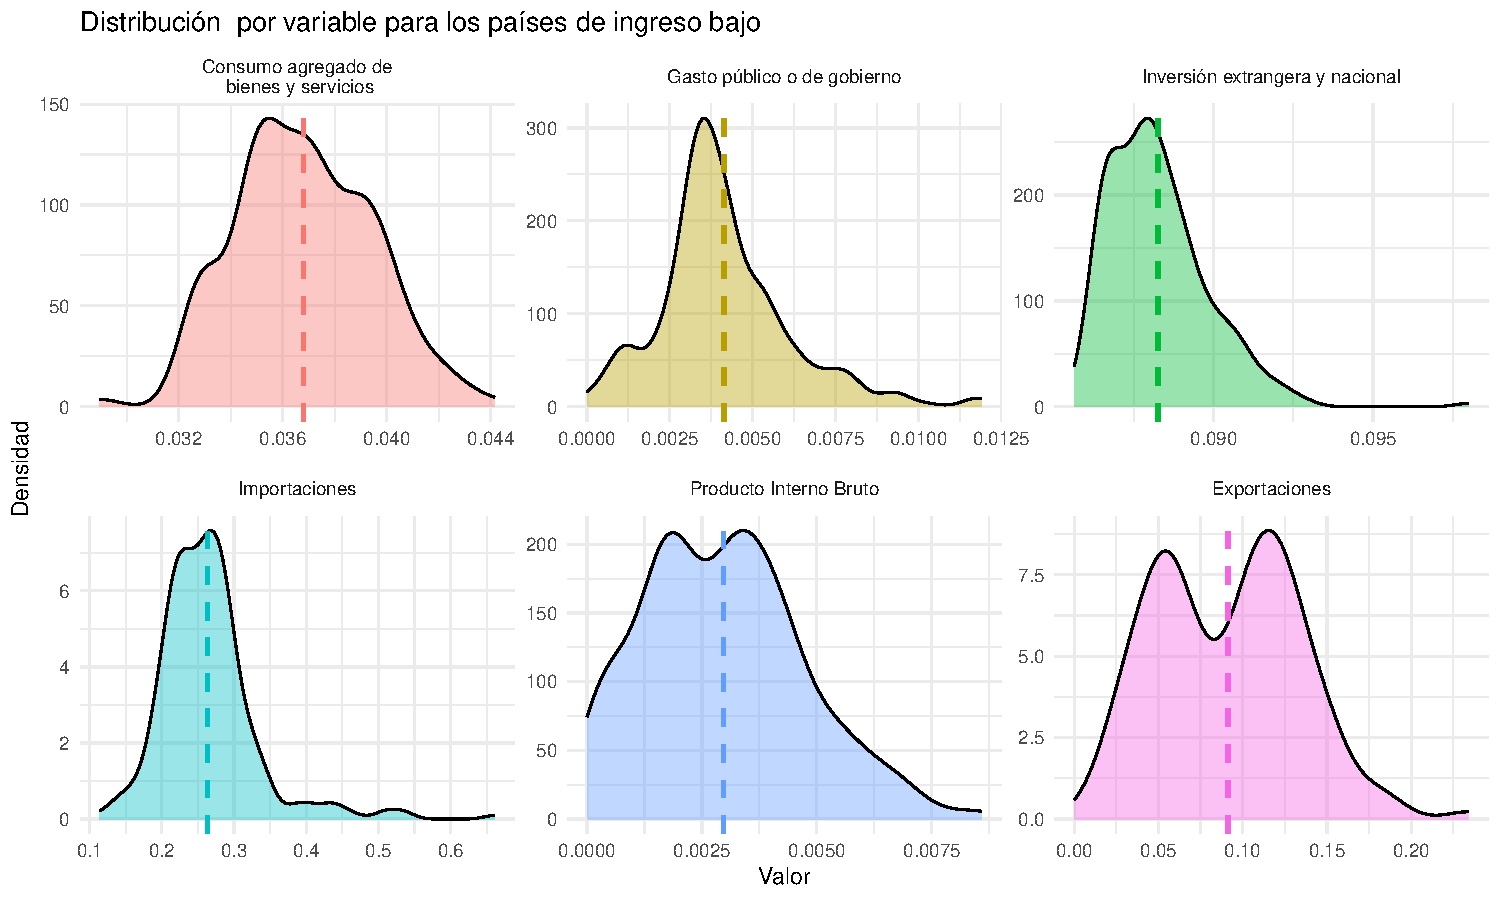
\includegraphics[width=1\linewidth]{figures/grafico_kde_bajo.pdf}
    \caption{Distribución de las variables para los países del grupo de ingreso bajo}
    \label{fig:KDE_bajo}
\end{figure}

\begin{figure}[H]
    \centering
    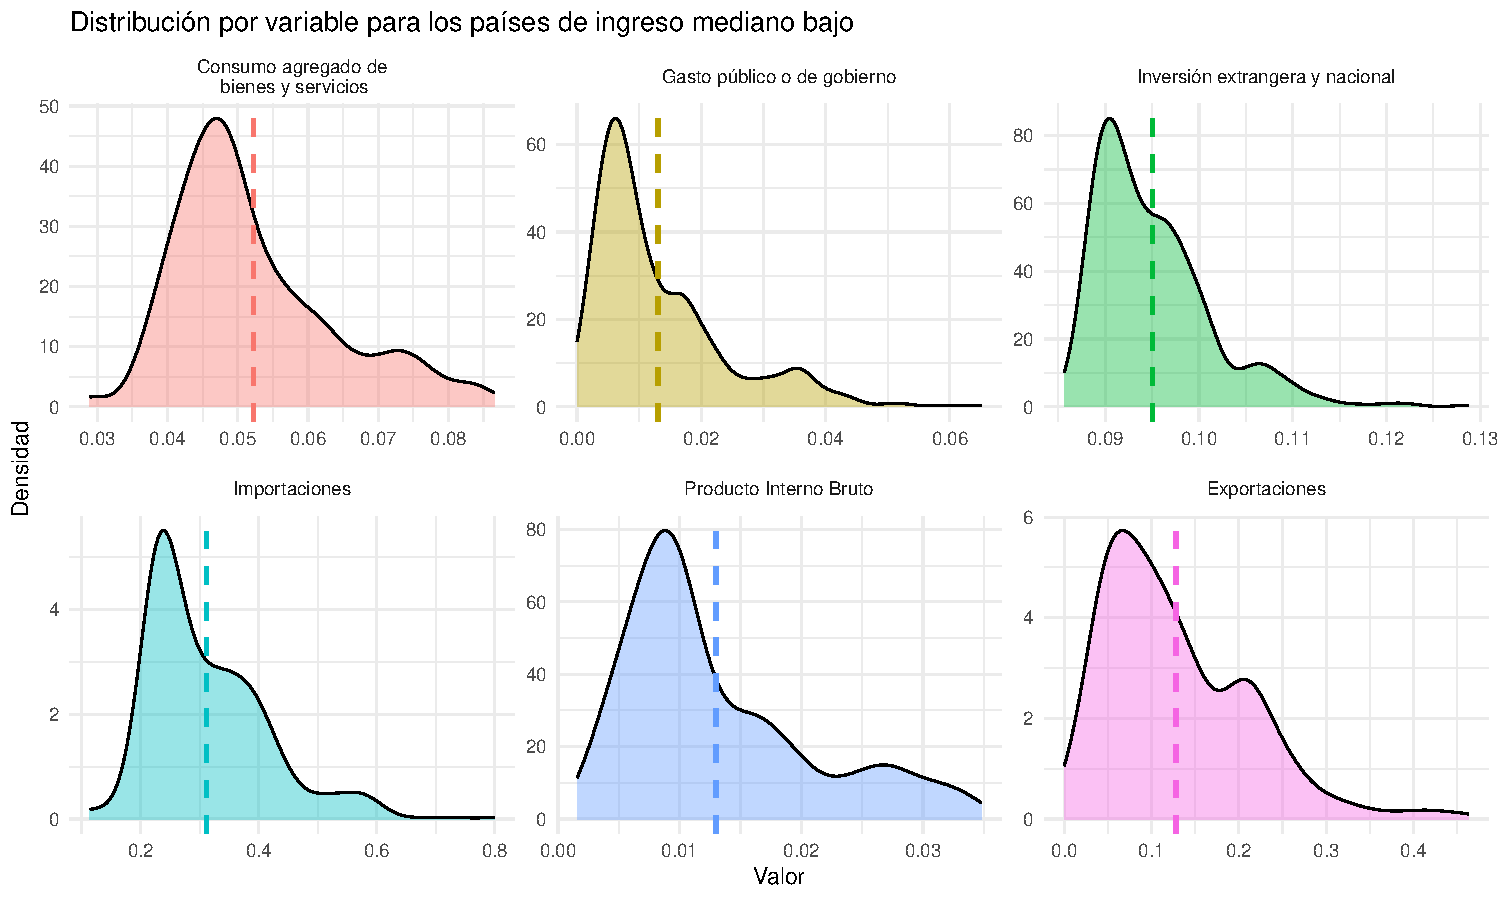
\includegraphics[width=1\linewidth]{figures/grafico_kde_mediobajo.pdf}
    \caption{Distribución de las variables para los países del grupo de ingreso mediano bajo}
    \label{fig:KDE_mediobajo}
\end{figure}

\begin{figure}[H]
    \centering
    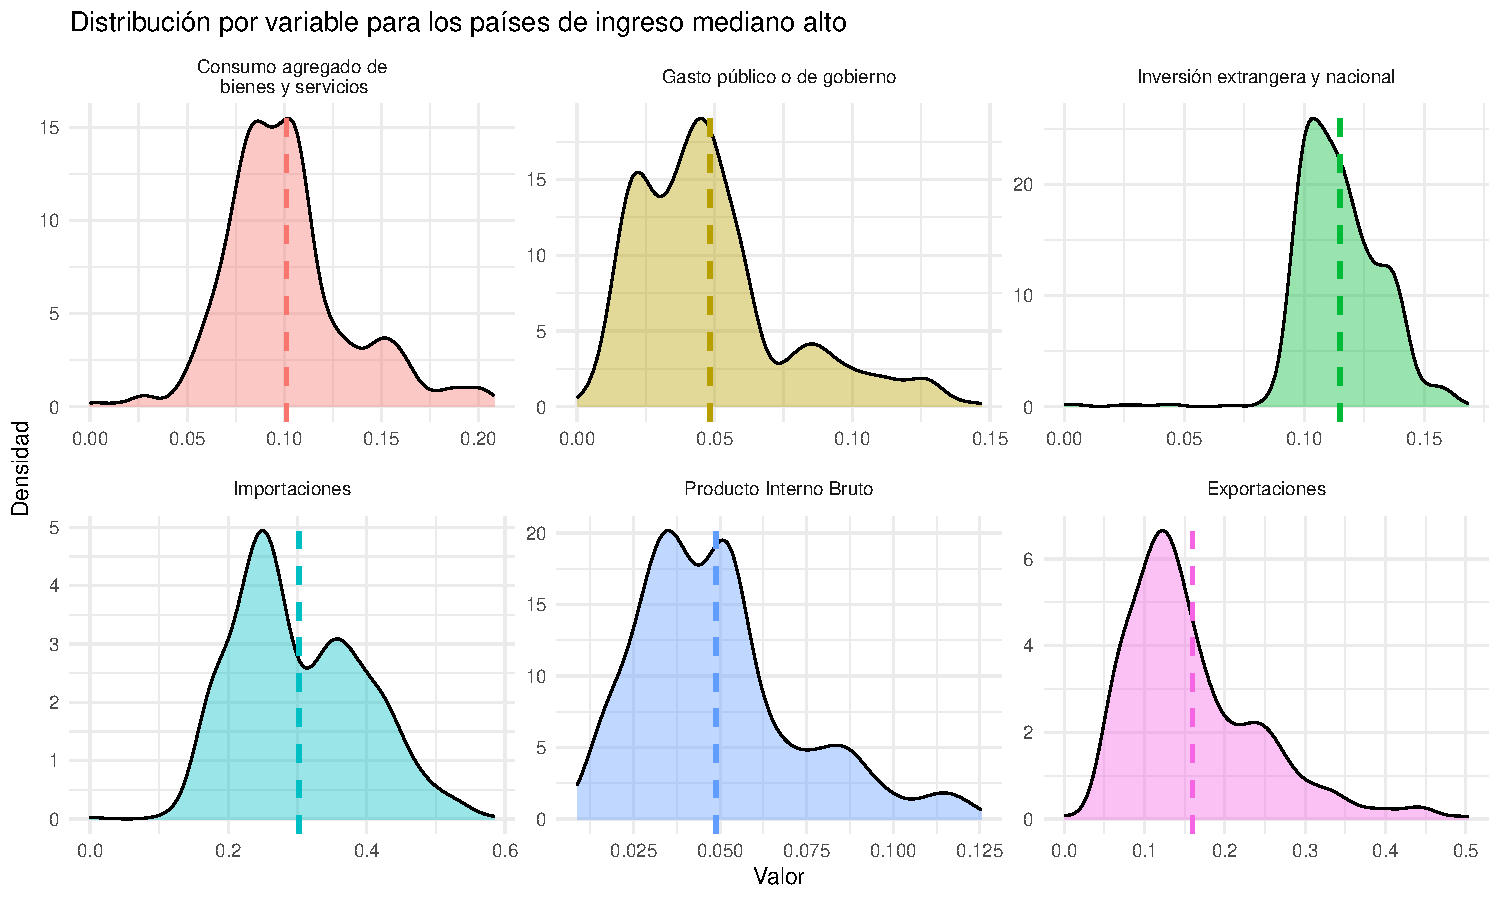
\includegraphics[width=1\linewidth]{figures/grafico_kde_medioalto.pdf}
    \caption{Distribución de las variables para los países del grupo de ingreso mediano alto}
    \label{fig:KDE_medioalto}
\end{figure}

\begin{figure}[h]
    \centering
    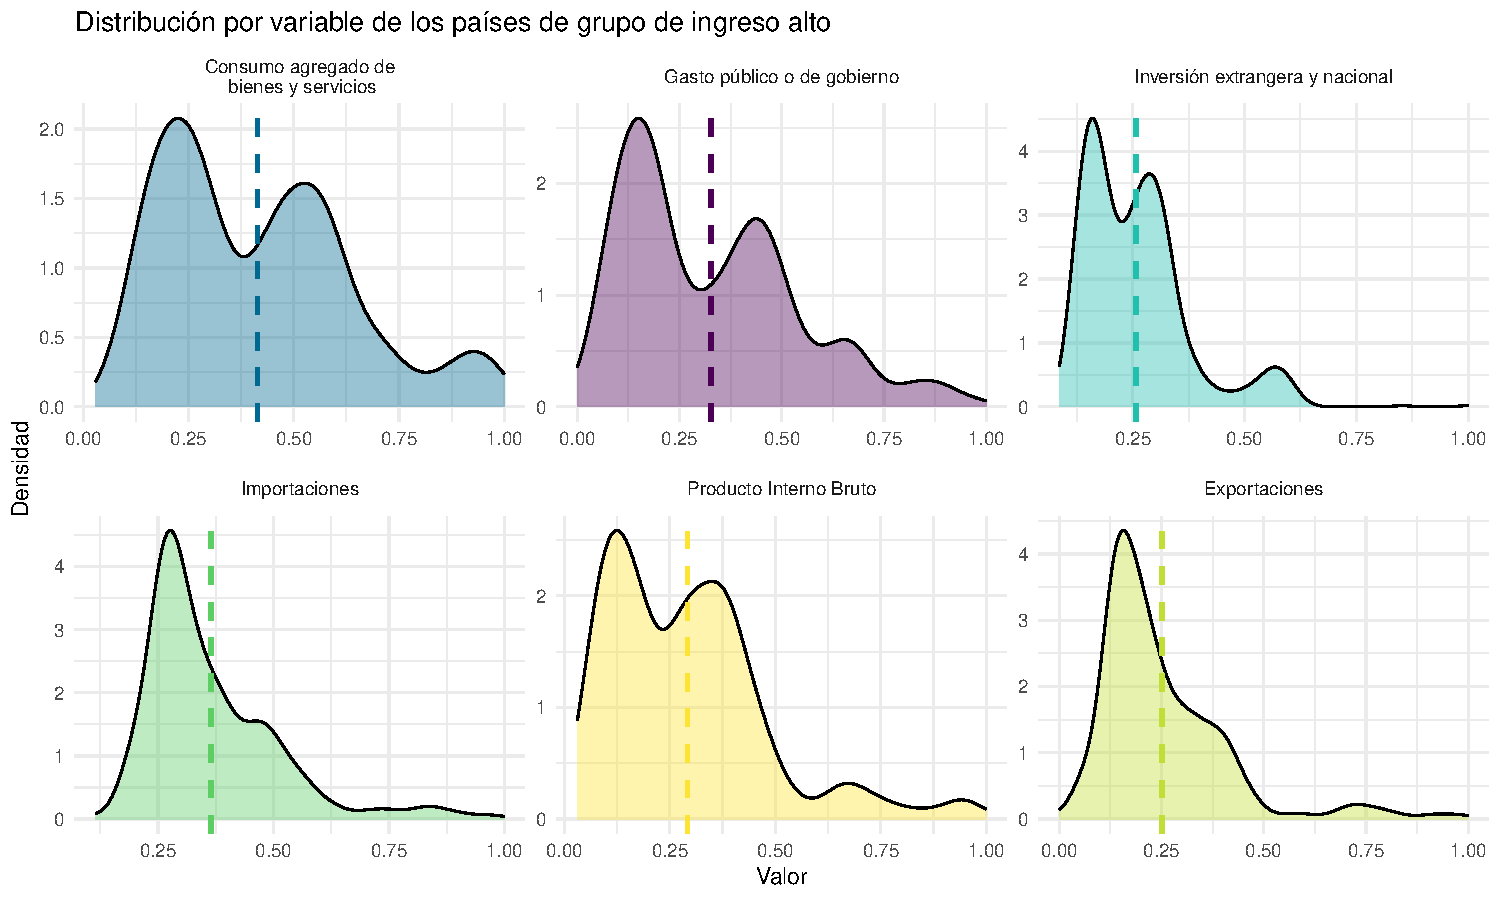
\includegraphics[width=1\linewidth]{figures/grafico_kde_alto.pdf}
    \caption{Distribución de las variables para los países del grupo de ingreso alto}
    \label{fig:KDE_alto}
\end{figure}

% \begin{table}[ht]
% \scriptsize
% \begin{tabular}{|c|l|l|l|l|l|l|}
% \hline
% \multicolumn{1}{|l|}{Variable} & Kolmogorov & General  & Alto     & Medio alto & Medio bajo & Bajo      \\ \hline
% \multirow{2}{*}{G}             & Coef       & 0.2355   & 0.14094  & 0.12482    & 0.16065    & 0.11816   \\ \cline{2-7} 
%                                & Val p      & 0.00     & 0.00     & 0.00       & 7.10E-14   & 0.0006433 \\ \hline
% \multirow{2}{*}{C}             & Coef       & 0.22     & 0.11168  & 0.1117     & 0.13251    & 0.046631  \\ \cline{2-7} 
%                                & Val p      & 2.20E-16 & 0.00     & 0.00       & 0.00       & 0.5583    \\ \hline
% \multirow{2}{*}{I}             & Coef       & 0.23159  & 0.095632 & 0.081562   & 0.098049   & 0.080039  \\ \cline{2-7} 
%                                & Val p      & 2.20E-16 & 0.00     & 0.0001383  & 0.02       & 0.04994   \\ \hline
% \multirow{2}{*}{M}             & Coef       & 0.11341  & 0.13539  & 0.10155    & 0.12196    & 0.12235   \\ \cline{2-7} 
%                                & Val p      & 2.20E-16 & 2.20E-16 & 0.00       & 0.00       & 0.0003603 \\ \hline
% \multirow{2}{*}{X}             & Coef       & 0.1288   & 0.13568  & 0.12738    & 0.10207    & 0.091368  \\ \cline{2-7} 
%                                & Val p      & 2.20E-16 & 2.20E-16 & 0.00       & 0.01       & 0.01632   \\ \hline
% \multirow{2}{*}{PIB}           & Coef       & 0.23162  & 0.090303 & 0.10752    & 0.15886    & 0.070574  \\ \cline{2-7} 
%                                & Val p      & 2.20E-16 & 1.45E-07 & 0.00       & 0.00       & 0.1135    \\ \hline
% \end{tabular}
% \end{table}

Una vez visualizado el comportamiento de nuestras variables, es posible intuir que nuestro conjunto de datos tiene un comportamiento no estacionario, osea que son no paramétricos, sin embargo, es necesaria la aplicación pruebas de normalidad, así como la visualización de su distribución para la comprobación de dicha sospecha.

La prueba de normalidad aplicada fue la Kolmogorov-Smirnov, esto debido a la cantidad de observaciones que contiene nuestra base de datos, presentando los resultados tanto para la muestra general como para la segmentación de los países según su grupo de ingreso en la siguiente tabla, mostrando que independientemente del grupo que se estudie los datos son no paramétricos.

\begin{table}[h]
\tiny
\centering
\begin{tabular}{|c|l|l|l|l|l|l|}
\hline
\multicolumn{1}{|l|}{Variable} & Kolmogorov & General  & Alto     & Medio alto & Medio bajo & Bajo      \\ \hline
\multirow{2}{*}{G}             & Coef       & 2.36E-01 & 1.41E-01 & 1.25E-01    & 1.61E-01    & 1.18E-01   \\ \cline{2-7} 
                               & Val p      & 0.00     & 0.00     & 0.00       & 7.10E-14   & 6.43E-04 \\ \hline
\multirow{2}{*}{C}             & Coef       & 2.20E-01 & 1.12E-01 & 1.12E-01    & 1.33E-01    & 4.66E-02  \\ \cline{2-7} 
                               & Val p      & 2.20E-16 & 0.00     & 0.00       & 0.00       & 5.58E-01  \\ \hline
\multirow{2}{*}{I}             & Coef       & 2.32E-01 & 9.56E-02 & 8.16E-02    & 9.80E-02    & 8.00E-02  \\ \cline{2-7} 
                               & Val p      & 2.20E-16 & 0.00     & 1.38E-04    & 2.00E-02    & 4.99E-02  \\ \hline
\multirow{2}{*}{M}             & Coef       & 1.13E-01 & 1.35E-01 & 1.02E-01    & 1.22E-01    & 1.22E-01  \\ \cline{2-7} 
                               & Val p      & 2.20E-16 & 2.20E-16 & 0.00       & 0.00       & 3.60E-04  \\ \hline
\multirow{2}{*}{X}             & Coef       & 1.29E-01 & 1.36E-01 & 1.27E-01    & 1.02E-01    & 9.14E-02  \\ \cline{2-7} 
                               & Val p      & 2.20E-16 & 2.20E-16 & 0.00       & 1.00E-02    & 1.63E-02  \\ \hline
\multirow{2}{*}{PIB}           & Coef       & 2.32E-01 & 9.03E-02 & 1.08E-01    & 1.59E-01    & 7.06E-02  \\ \cline{2-7} 
                               & Val p      & 2.20E-16 & 1.45E-07 & 0.00       & 0.00       & 1.14E-01  \\ \hline
\end{tabular}
\end{table}


De igual manera, resulta relevante la correlación que presentan las variables entre sí, esto para rectificar que las variable independientes comparten una relación con nuestra variable dependiente, además de visualizarlo de manera gráfica en las figuras \ref{fig:serietot} y  \ref{fig:serieing}, donde se muestra como estas comparten una tendencia y/o comportamiento.

\begin{figure}[h]
    \centering
    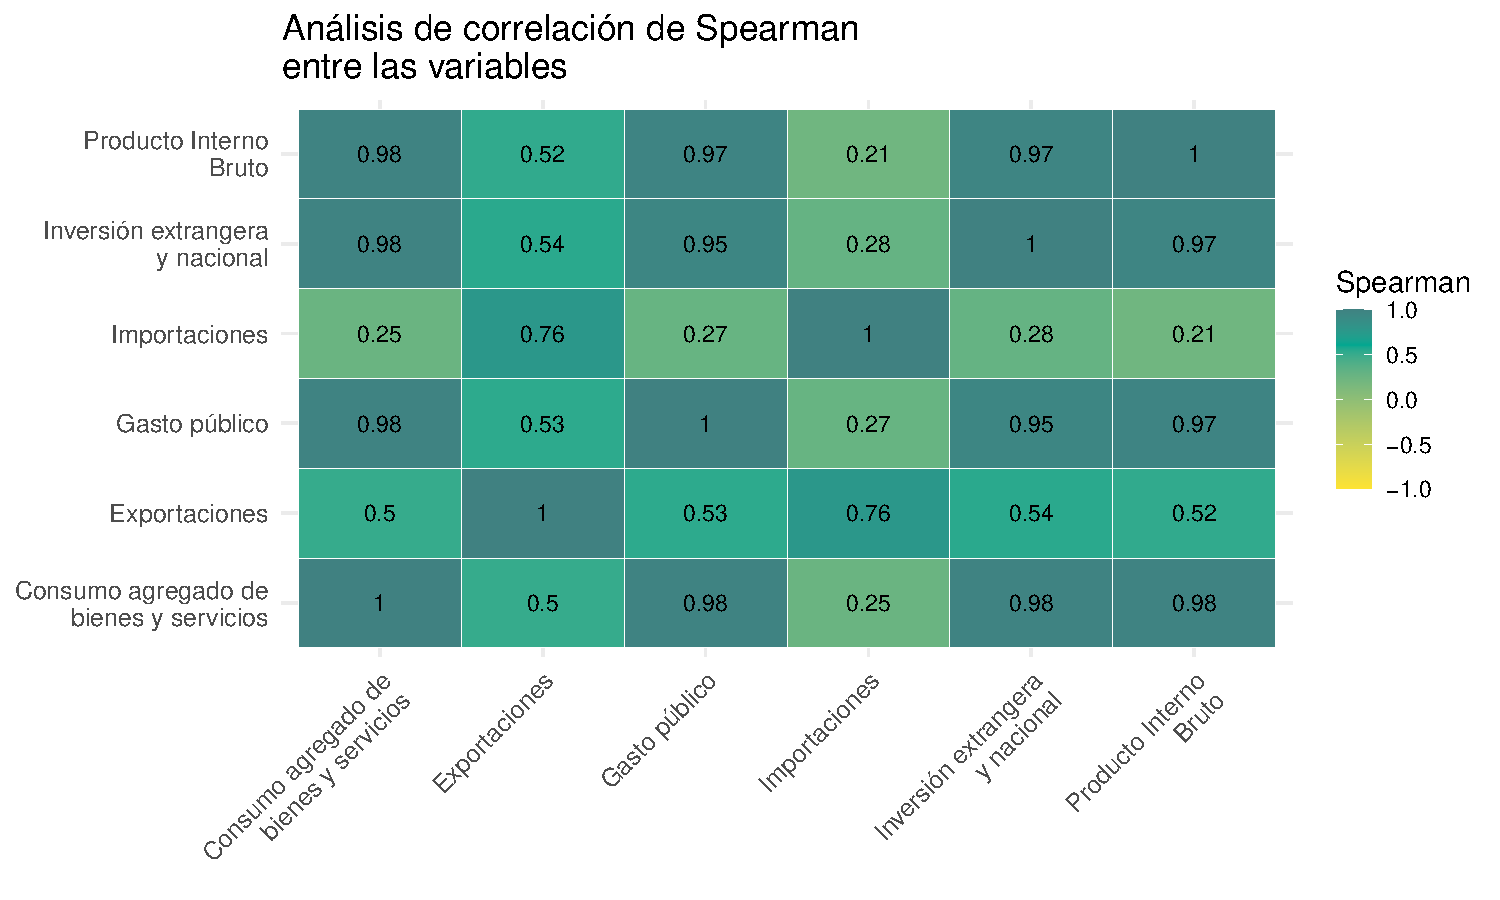
\includegraphics[width=1\linewidth]{figures/heatmap_spearman.pdf}
    \caption{Mapa de correlación de Spearman entre las variables}
    \label{fig:heatmap}
\end{figure}

\section{Conclusiones}


\section{Herramientas Utilizadas}

Todos los mapas, tablas y gráficos fueron generadas mediante R, más específicamente R Markdown, haciendo uso de las siguientes librerías:

\begin{multicols}{2}
    \begin{itemize} \footnotesize
      \item \texttt{C50}
      \item \texttt{caret}
      \item \texttt{dplyr}
      \item \texttt{e1071}
      \item \texttt{ggplot2}
      \item \texttt{readxl}
      \item \texttt{reshape2}
      \item \texttt{rnaturalearth}
      \item \texttt{rnaturalearthdata}
      \item \texttt{sf}
      \item \texttt{stats}
      \item \texttt{summarytools}
      \item \texttt{tidyr}
      \item \texttt{viridis}
    \end{itemize}
\end{multicols}

% \begin{itemize}
%     \item Librerias estadisticas descriptivas
%     \item Librerias mapas
%     \item Librerias correlación y heat maps
%     \item Librerias Dashboard
% \end{itemize}


% BIBLIOGRAFIA CON .bib

\printbibliography


% \begin{thebibliography}{00}
% \bibitem{b1} Formula 1 (2024). \textit{Everything you need to know about F1 – Drivers, teams, cars, circuits and more.}
% Recuperado el 11 de noviembre de 2024 de \url{https://www.formula1.com/en/latest/article/drivers-teams-cars-circuits-and-more-everything-you-need-to-know-about.7iQfL3Rivf1comzdqV5jwc}
% \end{thebibliography}

\end{document}
